\section{Results}\label{results}

\boldif{Results from interviews indicated that a common model of operating with merge conflicts exists.}
To understand how developers manage merge conflicts, we asked interview participants to describe their current processes for handling merge conflict.

\boldif{\textit{Add anecdotal quotes and descriptions from interviews to highlight these observations.}}
Participants talked about different steps that they follow, including using tools that alert them to potential or current merge conflicts, processes for analyzing and understanding conflicting code prior to implementing a resolution, and the use of tools for validating that their resolution worked.
As an example, P3 said:
\begin{quoting}
\textit{``Part of my job on the integration team requires that I check for bad regressions. I use scripts to track patches as they're being backported, so I know when and where to look if [a patch] introduces a conflict. [\ldots] And once I've fixed [the conflict], I try to compare with the previous version to make sure [the code] works in a similar way.''}
\end{quoting}

\boldif{Provide descriptions that link the stages of Merge Conflict model to this quote. Use it to drive description of simplified model description paragraph}

\boldif{Based on these anecdotal observations, we construct an initial model of the processes that developers employ when working with merge conflicts, see Fig.~\ref{model}.}
Our interview and survey results suggest that developers follow a series of phases through which they manage the life-cycle of individual merge conflicts.
We construct a model of the developer processes for managing merge conflicts and examine each phase in detail.
Figure~\ref{model} provides an illustration of this model. 
It consists of four phases: \emph{awareness, planning, resolution,} and \emph{evaluation.}

\boldif{Discuss the fact that no other studies have shown that a model exists for merge conflicts}

\begin{figure}[!htbp]
\centering
\fbox{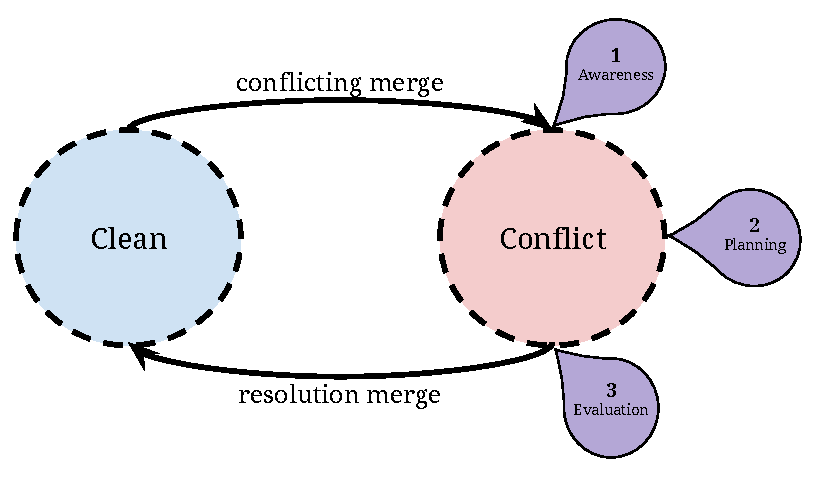
\includegraphics[width=0.90\textwidth,keepaspectratio]{imgs/MergeConflictModel}}
\caption{Model of Developer Processes for Managing Merge Conflicts. Developers alternate between \textit{clean} and \textit{conflicting} states of code. Beginning from (1)~\textit{development}, developers maintain (2)~\textit{awareness} of conflicts within the codebase in different ways. Once aware, developers begin (3)~\textit{planning} for a (4)~\textit{resolution} to fix the conflict. And finally, developers (5)~\textit{evaluate} the effectiveness of their deployed resolutions (returning to \emph{planning} if the resolution failed).\vspace*{-0.3\baselineskip}}
\label{model}
\end{figure}

\boldif{Awareness is how developers become aware}
First, the \emph{awareness} phase consists of the actions developers take to become aware of merge conflicts.
This could be passive, as the developer will become aware of a merge conflict when attempting to merge changes or perform a pull.
At the other end of the spectrum are developers who \emph{proactively} monitor for merge conflicts as they write code.
They are actively looking for changes that might be problematic, either manually or through the use of specialized tools.

\boldif{Planning is when developers plan their future actions}
Second, the \emph{planning} phase occurs after the developer has become aware that a conflict has occurred, and they are about to tackle the conflict.
This includes the decision of when they will try and resolve the conflict.
Some developers might try and resolve it immediately, while others might postpone the resolution.
Some might change their strategy depending on the conflict, incoming deadlines, or availability of resources.
This also includes other actions, such as if they are going to tackle the conflict alone, or collaborate with other developers knowledgeable in the area of conflict~\cite{CostaSarma}.

\boldif{Resolution is the action of implementing a resolution. Mundane and well understood, so we focus on the other three.}
Third, the \emph{resolution} phase represents the implementation of the planned resolution.
Several tools exist that help in this phase~\cite{nishimura,mens2002state,Brun2011}.
Here we focus on the difficulties that developers face during these resolution implementations (see Section~\ref{RQ2}).

\boldif{Evaluation is how developers check that their solution is correct}
Finally, after the conflict has been resolved, developers enter in the \emph{evaluation} phase.
In this phase, the developer has to evaluate their resolution before considering the conflict as resolved.
This is to ensure the correctness of the resulting code.
Possible actions during this stage includes compiling the source code.
Developers wanting more guarantees can go a step further and run the tests.
Finally, some groups have policies such as code reviews that need to be performed on the merge conflict resolution.
 
\boldif{To explore and validate this model, we asked developers to reflect upon how they become aware of merge conflicts, how they plan for merge conflict resolutions, and how they evaluate their resolutions in the \textit{Processes Survey}.}
In order to explore and validate this model, and our assumptions, we conducted the \emph{Processes Survey}.
Our aim in this survey was to understand how developers become aware of merge conflicts (what steps they take, what tools they use, etc.).
Also, we wanted to investigate their strategies for dealing with merge conflicts and how they decide whether the resolution has addressed all of their concerns.

Results are categorized according to the life-cycle of merge conflicts; with specific results for the \textit{awareness} (Section~\ref{RQ1}), \textit{planning} (Section~\ref{RQ2}), and \textit{evaluation} phases (Section~\ref{RQ3}).
We then present the difficulties that developers experience when managing merge conflicts (Section~\ref{RQ4}).
And finally, we examine the gaps in tool support for managing merge conflicts according to developer's needs (Section~\ref{RQ5}).